\newpage
\section{Musique}

\begin{figure}[h]
    \centering
    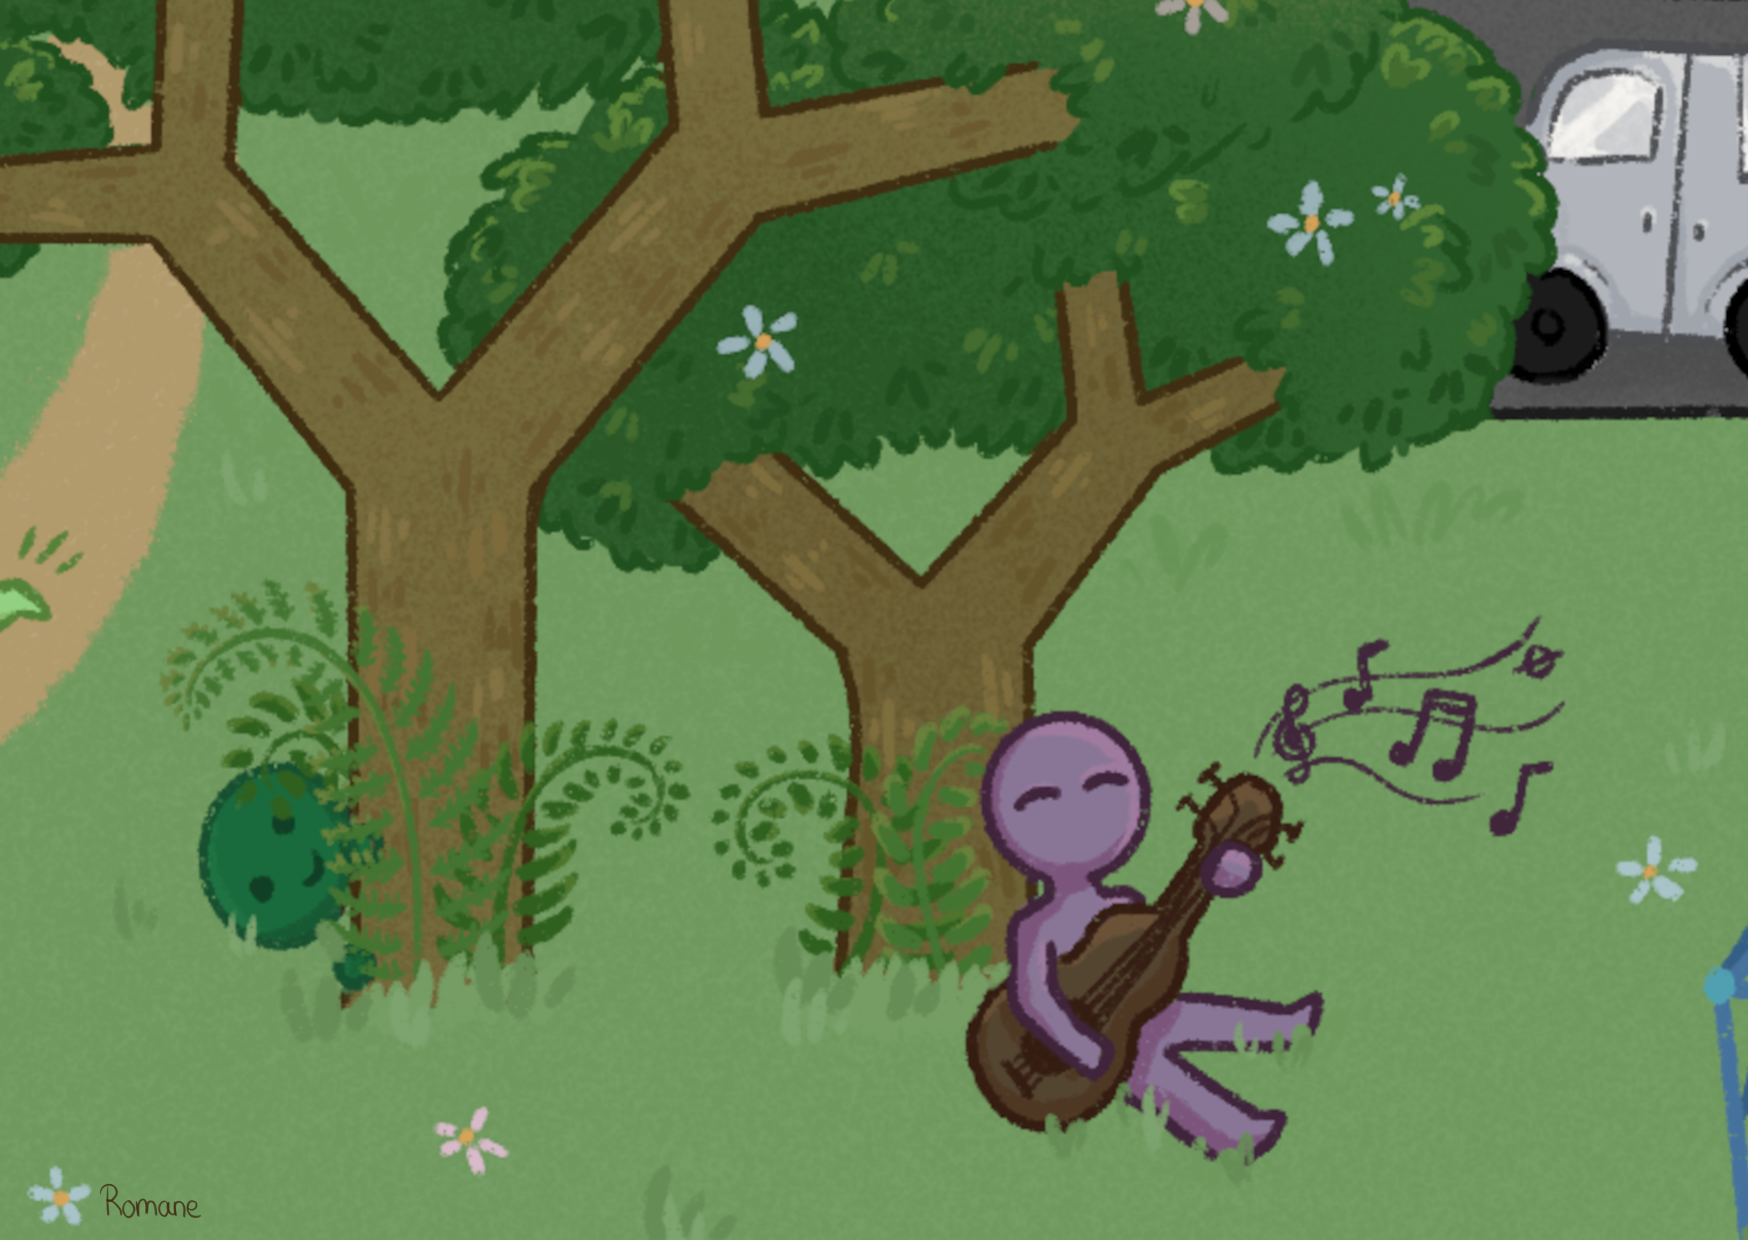
\includegraphics[height=0.5\textheight]{Cartes_postales/carte06-musique.png}\label{fig:c06}
    \caption{Carte postale: Musique}
\end{figure}

Sais-tu que la musique que nous écoutons repose sur un conflit mathématique insoluble? Une note de musique est une vibration de l'air, et deux notes sont harmonieuses si le rapport de leurs fréquences est une fraction simple: le rapport $2$ correspond à l'octave, tandis que le rapport $3/2$ définit la quinte. Pour construire une échelle musicale, une gamme, on cherche donc à utiliser ces deux intervalles. Cependant, en accumulant douze quintes successives, on obtient une valeur très proche mais différente de sept octaves cumulées: \[(3/2)^{12} \approx 129,746, \text{alors que } 2^7 = 128.\]

Cette infime différence, appelée le comma pythagoricien, empêche les cycles de notes de se refermer parfaitement, ce qui crée inévitablement des dissonances à l'oreille. En pratique, comme il est impossible d'obtenir une gamme où toutes les quintes et toutes les octaves sont parfaitement pures, les musiciens ont dû faire un compromis: la "gamme tempérée". En multipliant la fréquence de chaque note par un coefficient fixe de $2^{1/12}$, on répartit équitablement cette dissonance sur les douze notes de la gamme. En couplant cette théorie mathématique à notre système occidental, on accepte que les notes ne sonnent jamais de manière absolument pure, mais on réussit à éviter tout accord trop faux, permettant aux instruments de jouer harmonieusement dans toutes les tonalités.